This supplementary material offers additional results, comprehensive dataset information, and thorough analyses that bolster the findings and conclusions outlined in the main text. It is organized as follows:

\begin{itemize}
\item Additional qualitative results. 
\item User Study with DiT-based methods.
\item Data pre-processing method. %(Section \ref{sup.data-proc})
\item Dataset details, regarding total quantity, total durations, etc. %(Section \ref{sup.data-detail})
\item Prompt refinement method. %(Section \ref{sup.prompt})
\item Motion VAE training.
\end{itemize}

\section{Qualitative Comparisons}\label{sup.results}

While the main text focuses on quantitative comparisons with the motion-controllable video generation models and ablation studies on different designs for Trajectory Extractor and Motion-guidance Fuser, here we provide further visual comparisons.

% \subsection{Compare with motion-controllable methods}

\begin{figure*}[!ht]
    \centering
    \includegraphics[width=\textwidth]{images/compare_opensora.pdf}
    \caption{
        Qualitative comparison between Tora and OpenSora. All results are generated under the same text and image conditions. Tora employs an appropriate trajectory that simulates real-world physics, leading to more coherent and stable motion.
    }
    \label{sup.f.opensora}   
\end{figure*}

% Figure~\ref{fig:compare} provides a comparative analysis of our proposed method against mainstream motion control techniques. In the first scenario involving the coordinated movement of two individuals, all methods manage to generate motion trajectories that are relatively accurate. However, our approach stands out for its superior visual quality. This advantage is largely attributed to the use of longer sequence frames, which contribute to smoother motion trajectories and more realistic background rendering. For example, in our generated bicycle scenario, the human legs exhibit lifelike pedaling motions, while the output from DragNUWA shows legs that appear to float almost horizontally, compromising physical realism. Moreover, both DragNUWA and MotionCtrl encounter significant motion blur towards the end of their videos. Additionally, MotionCtrl introduces unintended camera movements during the riding sequence, despite the absence of any intended camera movement conditions. In another instance, DragNUWA suffers from severe deformation of the lantern as the provided trajectory oscillates up and down. Although MotionCtrl's trajectory is relatively accurate, the resulting video does not align with the expected portrayal of two lanterns. Overall, our method not only adheres closely to the provided trajectories but also minimizes object deformation, thereby ensuring higher fidelity in motion representation.


\subsection{Compare with OpenSora}

Despite OpenSora's impressive accomplishments, it faces challenges when creating long videos featuring complex motions, such as simultaneous movement of multiple objects, swinging, or circling. This often leads to incoherent or distorted foreground objects, negatively impacting visual quality. To our delight, we discovered that incorporating appropriate trajectory control into the DiT model offers a more effective constraining signal. This improvement markedly enhances video fluidity and preserves object fidelity, as demonstrated in Figure ~\ref{sup.f.opensora}.

\begin{figure*}[!ht]
    \centering
    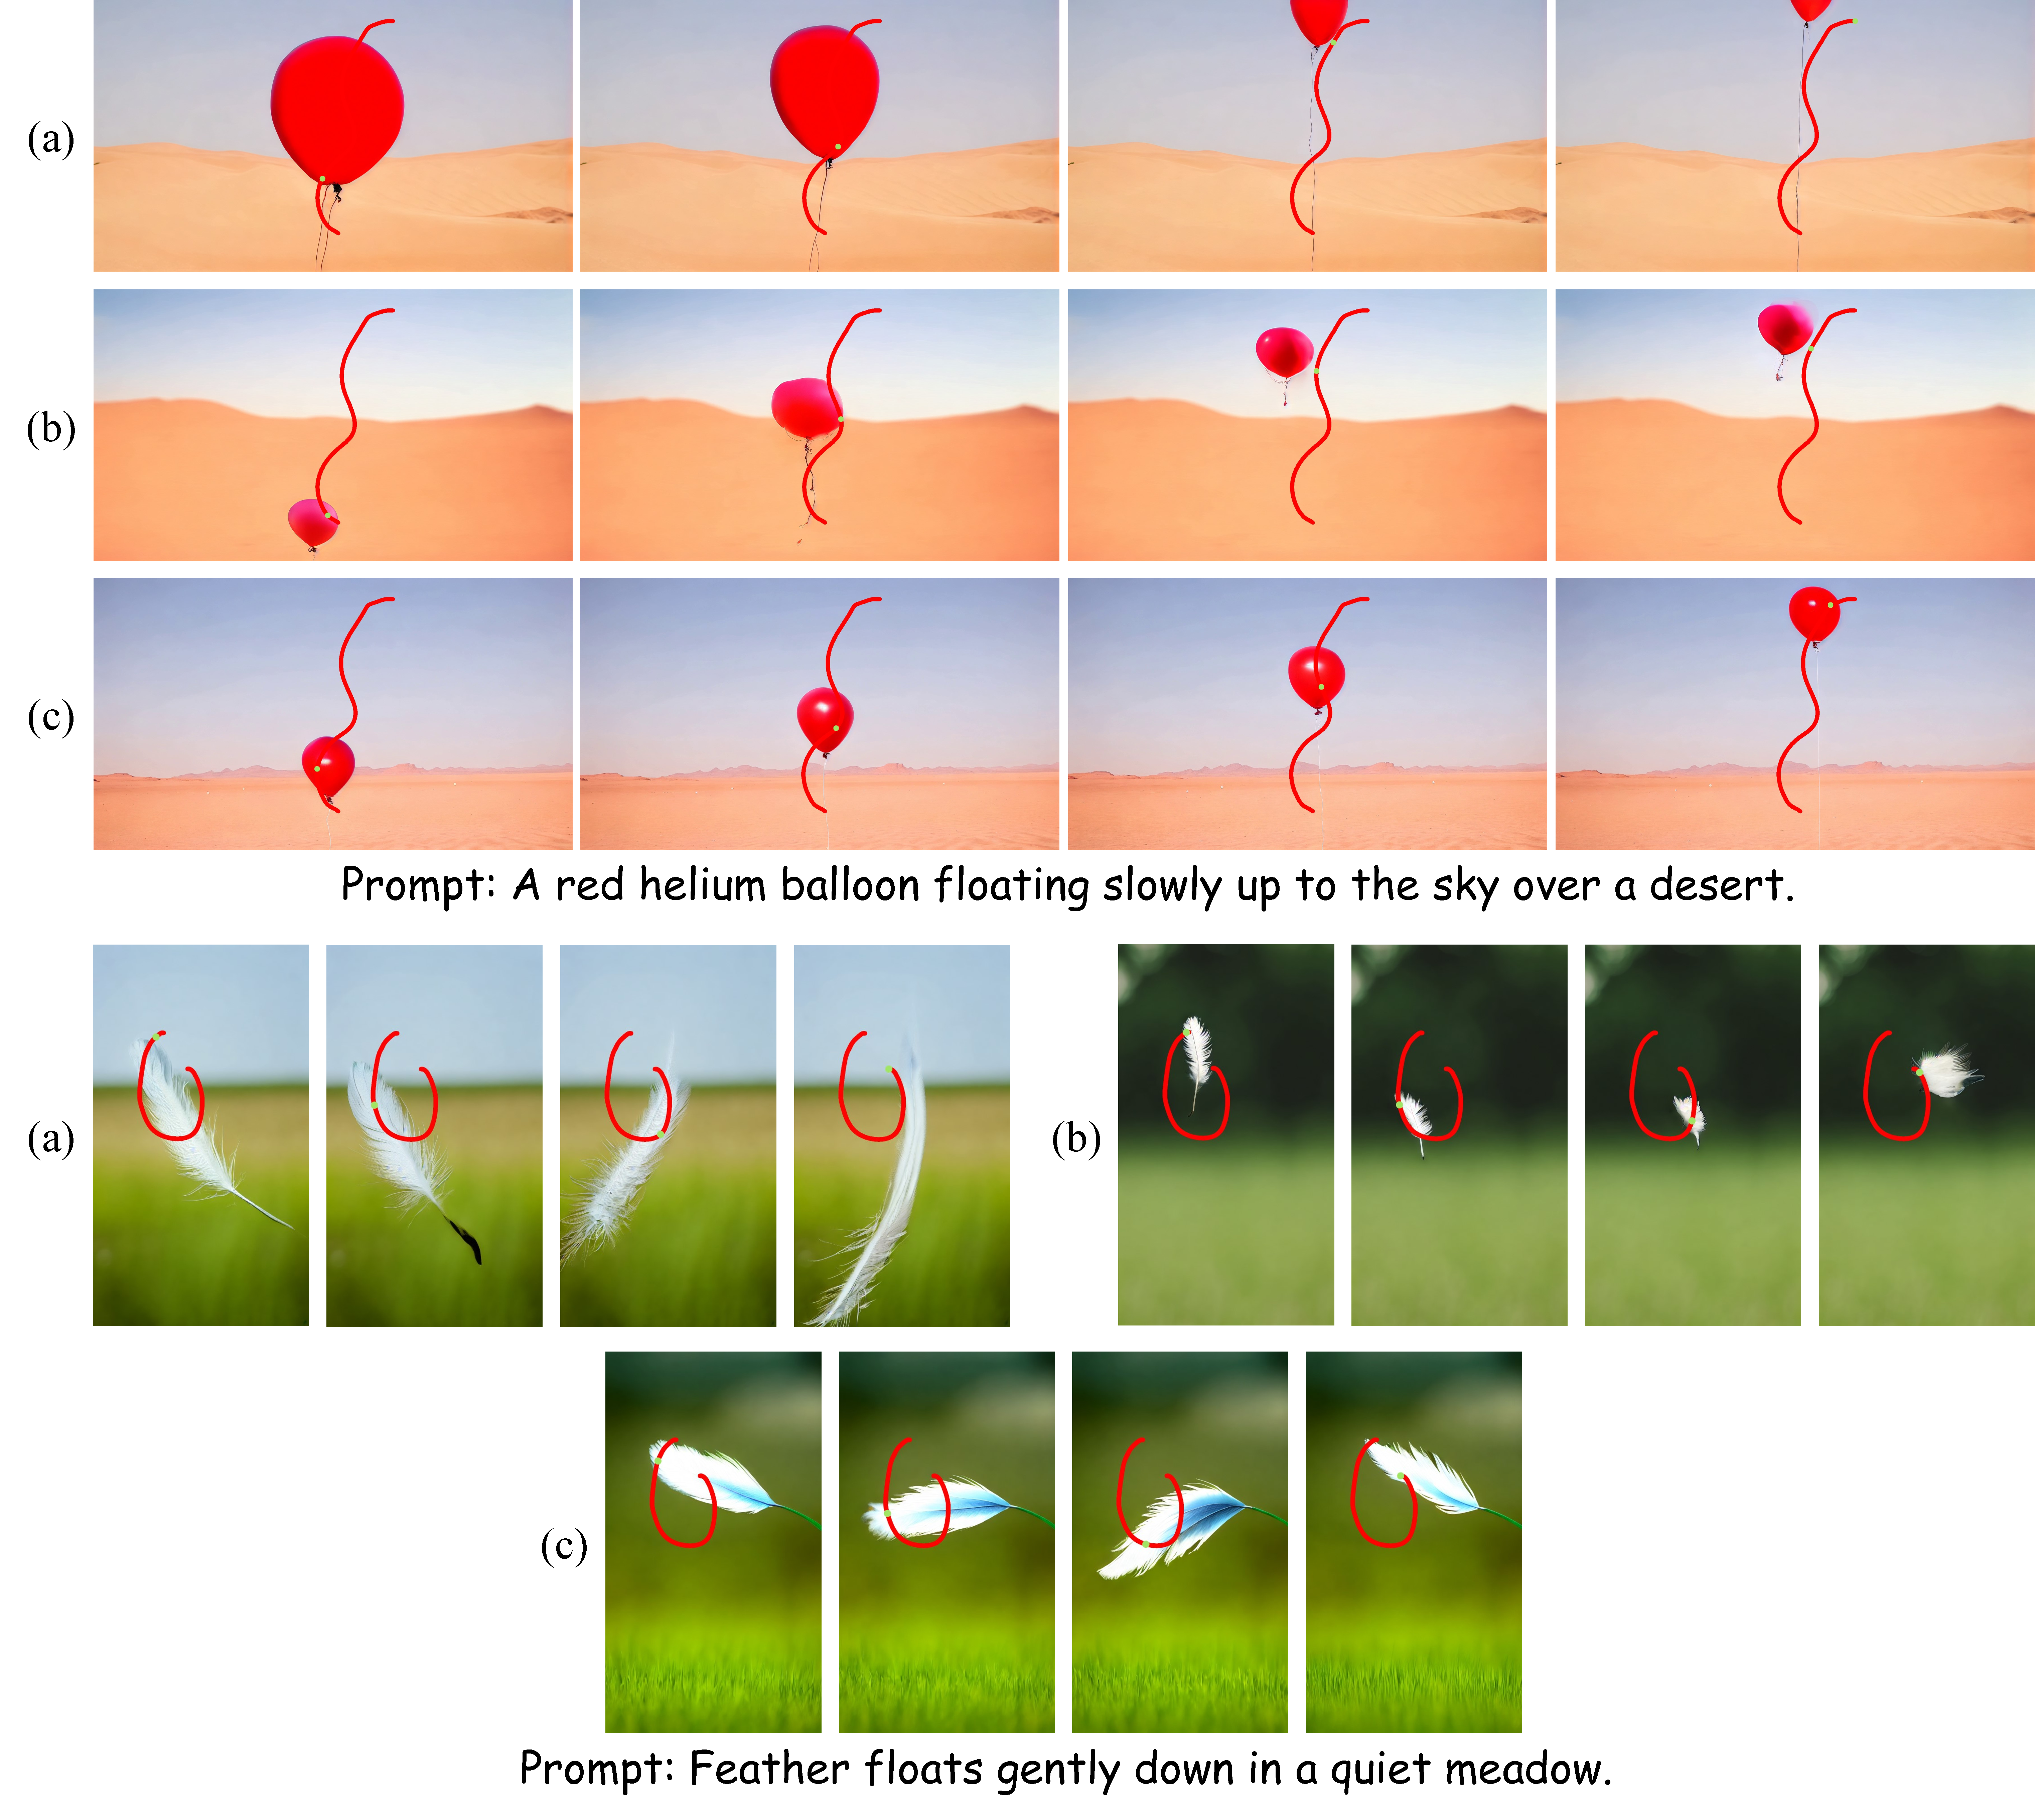
\includegraphics[width=\textwidth]{images/compare_compression.pdf}
    \caption{
        Generated videos employing different trajectory compression methods: (a) Sampling Keyframe; (b) Average Pooling; (c) 3D VAE.
    }
    \label{sup.f.compress}   
\end{figure*}

In scenarios where a teddy bear is oscillating side to side on a skateboard or a rose is swirling in circular motions, OpenSora, which relies solely on textual directives for motion control, exhibits noticeable object deformations. In contrast, Tora excels at maintaining the inherent shape of the objects. Additionally, when managing the motion of multiple entities, such as a pair of jellyfish—one moving upward while the other moves downward, OpenSora demonstrates noticeable flickering, underscoring its limitations in handling complex movements. In conclusion, the integration of Tora's motion signaling mechanism enhances both the controllability and stability of the synthesized video output.

\subsection{Comparison of Different Trajectory Compression Methods}
We train our proposed trajectory extractor using the various trajectory compression methodologies previously discussed. The comparisons of these methods are visually illustrated in Figure \ref{sup.f.compress}.



\begin{figure*}[!ht]
    \centering
    % 第一张图
    \begin{subfigure}[c]{0.3\textwidth}
        \centering
        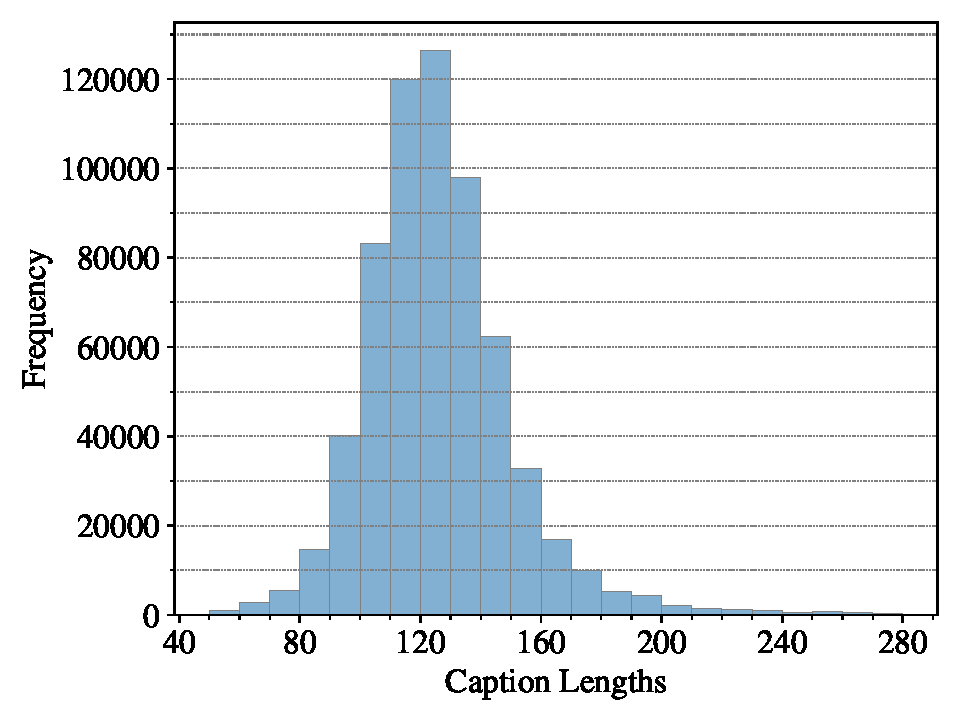
\includegraphics[width=\linewidth]{images/Caption_Lengths.pdf}
        \caption{Histogram of Caption Lengths.}
        \label{sup.f.hist1}
    \end{subfigure}%
    \hfill
    % 第二张图
    \begin{subfigure}[c]{0.3\textwidth}
        \centering
        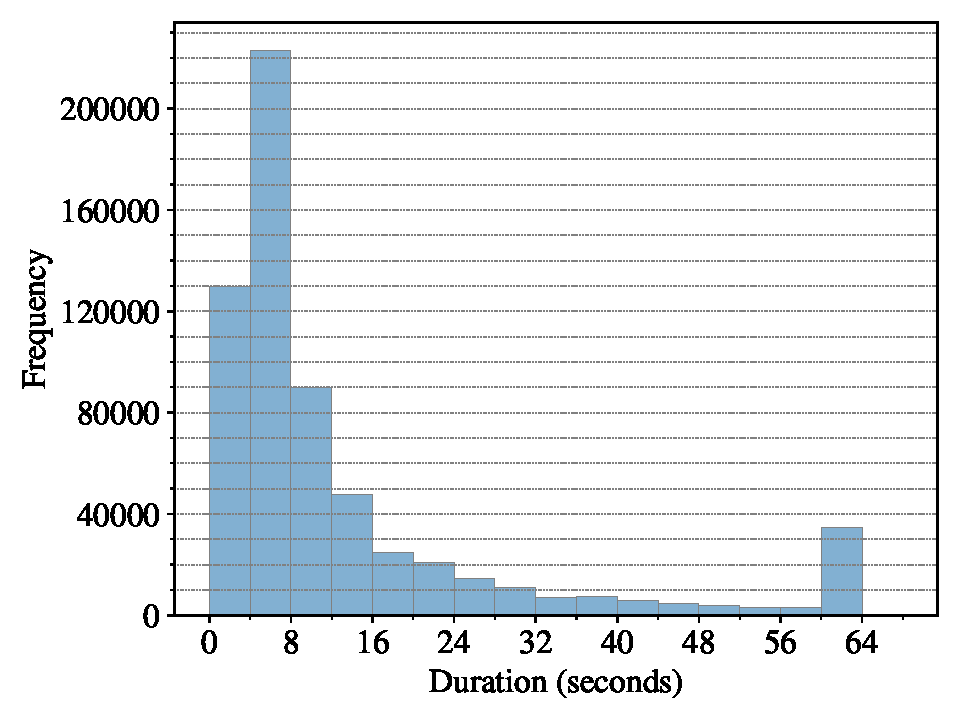
\includegraphics[width=\linewidth]{images/Duration.pdf}
        \caption{Histogram of Video Durations.}
        \label{sup.f.hist2}  
    \end{subfigure}%
    \hfill
    % 第三张图
    \begin{subfigure}[c]{0.3\textwidth}
        \centering
        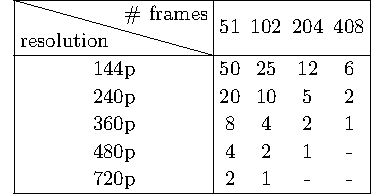
\includegraphics[width=\linewidth]{images/bucket.pdf}
        \caption{The training batch size of every bucket (resolution, duration).}
        \label{sup.f.bucket}   
    \end{subfigure}
    
    \caption{Overview of the training data distributions and batch sizes.}
    \label{fig:combined}
\end{figure*}

In key-frame sampling, while it successfully captures essential motion, it frequently leads to misalignment between video patches and motion patches, especially during rapid motion sequences. This misalignment hinders the generated objects from accurately tracking their trajectories, negatively impacting visual fluidity and overall quality. On the other hand, average pooling smooths out minor variations, resulting in a more consistent motion representation. However, in complex trajectories, such as S-shaped turns where consecutive frame directions are inconsistent, this approach may introduce artifacts because the physical relevance of optical flow decreases. In contrast, our proposed 3D VAE approach effectively compresses trajectory information into the video's latent space. By training the 3D VAE on the large dataset with flow annotations, it successfully extracts the most relevant motion features for guidance, preserving the movement of successive frames to a significant extent. As evidenced in the results, this method significantly enhances the fluidity and coherence of the generated movements, producing visually compelling sequences that closely resemble natural motion.

\section{User Study with DiT-based methods}
We conduct a user study to compare OpenSora-v1.2, CogVideoX-2B~\cite{yang2024cogvideox}, Vidu~\cite{DBLP:journals/corr/abs-2405-04233}, and Kling v1.0~\cite{Kling}, assessing the effectiveness of our method using our evaluation dataset. 10 human volunteers participate in evaluating quality based on three criteria: physics simulation, sensory quality, and instruction adherence. For Tora, participants draw appropriate trajectories in response to given text prompts. The experiment employs a pairwise comparison approach, where evaluators choose the superior output from each pair of generated results based on the same input. The resulting win rates appear in Table \ref{sup.userstudy}. Our method outperforms both OpenSora and CogVideoX-2B across all metrics, affirming the superiority of our proposed modules and data processing methods. Compared to the closed-source method, Vidu, we achieve competitive results. Kling demonstrates remarkable capabilities, and we hope that Tora can work to close the performance gap in future iterations. 

\begin{table}[!ht]
\centering
\fontsize{8.0pt}{9.5pt}\selectfont
\begin{tabular}{cccc}
\toprule
Model          & Phys. Simu.  & Sens. Qual.  & Inst. Foll. \\ 
\midrule
Tora vs. OpenSora-v1.2 & 71\% & 61\% & 64\%     \\
Tora vs. CogVideoX  & 53\% & 56\% & 52\%     \\ 
Tora vs. Vidu  & 54\% & 48\% & 47\%     \\ 
Tora vs. Kling  & 45\% & 43\% & 41\%     \\ 
\bottomrule
\end{tabular}
\caption{Win rates of Tora compared to OpenSora-v1.2, CogVideoX, Vidu, and Kling in terms of Physics Simulation, Sensory Quality, and Instruction Following.}
\label{sup.userstudy} 
\end{table}



\section{Data Pre-processing}\label{sup.data-proc}

During the processing of the video datasets, constructing a high-quality training set is crucial as it significantly impacts the quality of the generated videos. The following is a detailed description of our data processing workflow, which includes steps such as invalid videos removal, resolution filtering, camera motion filtering, and assessing the degree of object motion.

Initially, during the dataset preparation phase, we remove invalid videos. This step aims to identify and discard videos that do not meet our established criteria, including those with encoding errors, a duration of zero, or low quality. We identify encoding errors and zero-duration videos by directly decoding them. Furthermore, we predict both the aesthetic score\footnote{https://github.com/christophschuhmann/improved-aesthetic-predictor} and the optical flow score~\cite{DBLP:journals/pami/XuZCRYTG23} for each video. A video is deemed valid only if its aesthetic score exceeds 5.5 and its flow score is greater than 3.

Next, we perform resolution filtering. To ensure the effectiveness of subsequent study, we establish a minimum resolution standard of 720p. By checking the resolution of each video, we can eliminate those that fall below this threshold, thereby ensuring that the videos in our dataset possess adequate clarity and detail.


Subsequently, we perform camera motion filtering using a camera motion detector\footnote{https://github.com/antiboredom/camera-motion-detector} and a motion segmentor ~\cite{DBLP:conf/eccv/ZhaoLGWL22} to filter out videos with significant camera movement, which may distort the model's ability to focus on the motion of the primary subjects. More specifically, the zoom detection threshold is set between 0.4 and 0.6. The detected camera movement angles, calculated based on the background from the motion segmentation results, are valid as follows:$[0^{\circ}, 20^{\circ}], [160^{\circ}, 200^{\circ}], [340^{\circ}, 360^{\circ}]$. 

Finally, we analyze the magnitude score of the optical flow within the foreground, excluding those scenes that are mostly static or exhibit minimal movement. Moreover, dramatic object motions in some videos can cause significant optical flow deviations, interfering with trajectory training. Consequently, we retain these videos with a probability of $(1 - flow\_score / 100)$. 

Through these rigorous filtering and processing steps, we successfully construct a high-quality video dataset suitable for subsequent training, providing a solid foundation for our study.

\section{Dataset Details}\label{sup.data-detail}

This section offers an overview of the dataset used in this study, covering its origin and composition. We employ histograms and descriptive statistics to illustrate the dataset's structure and distribution.

\subsection{Training Data}

The video data is sourced from the Panda-70M subset, Mixart, and internal videos. We initially collect 2.6M videos and apply the data preprocessing pipeline to filter the content, resulting in 631k eligible videos for training. An overview of the training dataset is presented in Table \ref{sup.t1}, which details the durations, resolution and FPS.

\begin{table}[!ht]
\centering
%\setlength{\tabcolsep}{2.5pt}
\renewcommand{\arraystretch}{1.1}
\begin{tabular}{lr}
\toprule
    \# Videos Clips &  631053 \\
    Total Durations (hours) &  2952.93  \\
    Average Shorter Edge Length  &  965.11 \\
    Average FPS   &  29.23     \\ 
\bottomrule
\end{tabular}
\caption{Statistical information about the training data.}
\label{sup.t1}
\end{table}

Additionally, Table \ref{sup.t2} summarizes the mean and standard deviation for the durations, number of frames, and caption lengths. We also present histogram to show the distribution of the caption lengths and the durations of all video clips, as shown in the Figure \ref{sup.f.hist1} and Figure \ref{sup.f.hist2}. 

\begin{table}[!ht]
\centering
%\setlength{\tabcolsep}{2.5pt}
\renewcommand{\arraystretch}{1.1}
\begin{tabular}{lrr}
\toprule
    & mean & std \\ 
\midrule
    Durations (seconds) &  16.85  &    19.58    \\
    \#Frames &  506.22   &  644.38 \\
    Caption Length (\#word)   &  125.52 &  24.22  \\ 
\bottomrule
\end{tabular}
\caption{Statistics of training set, regarding durations, number of frames, and caption lengths.}
\label{sup.t2}
\end{table}

\begin{figure*}[!ht]
    \centering
    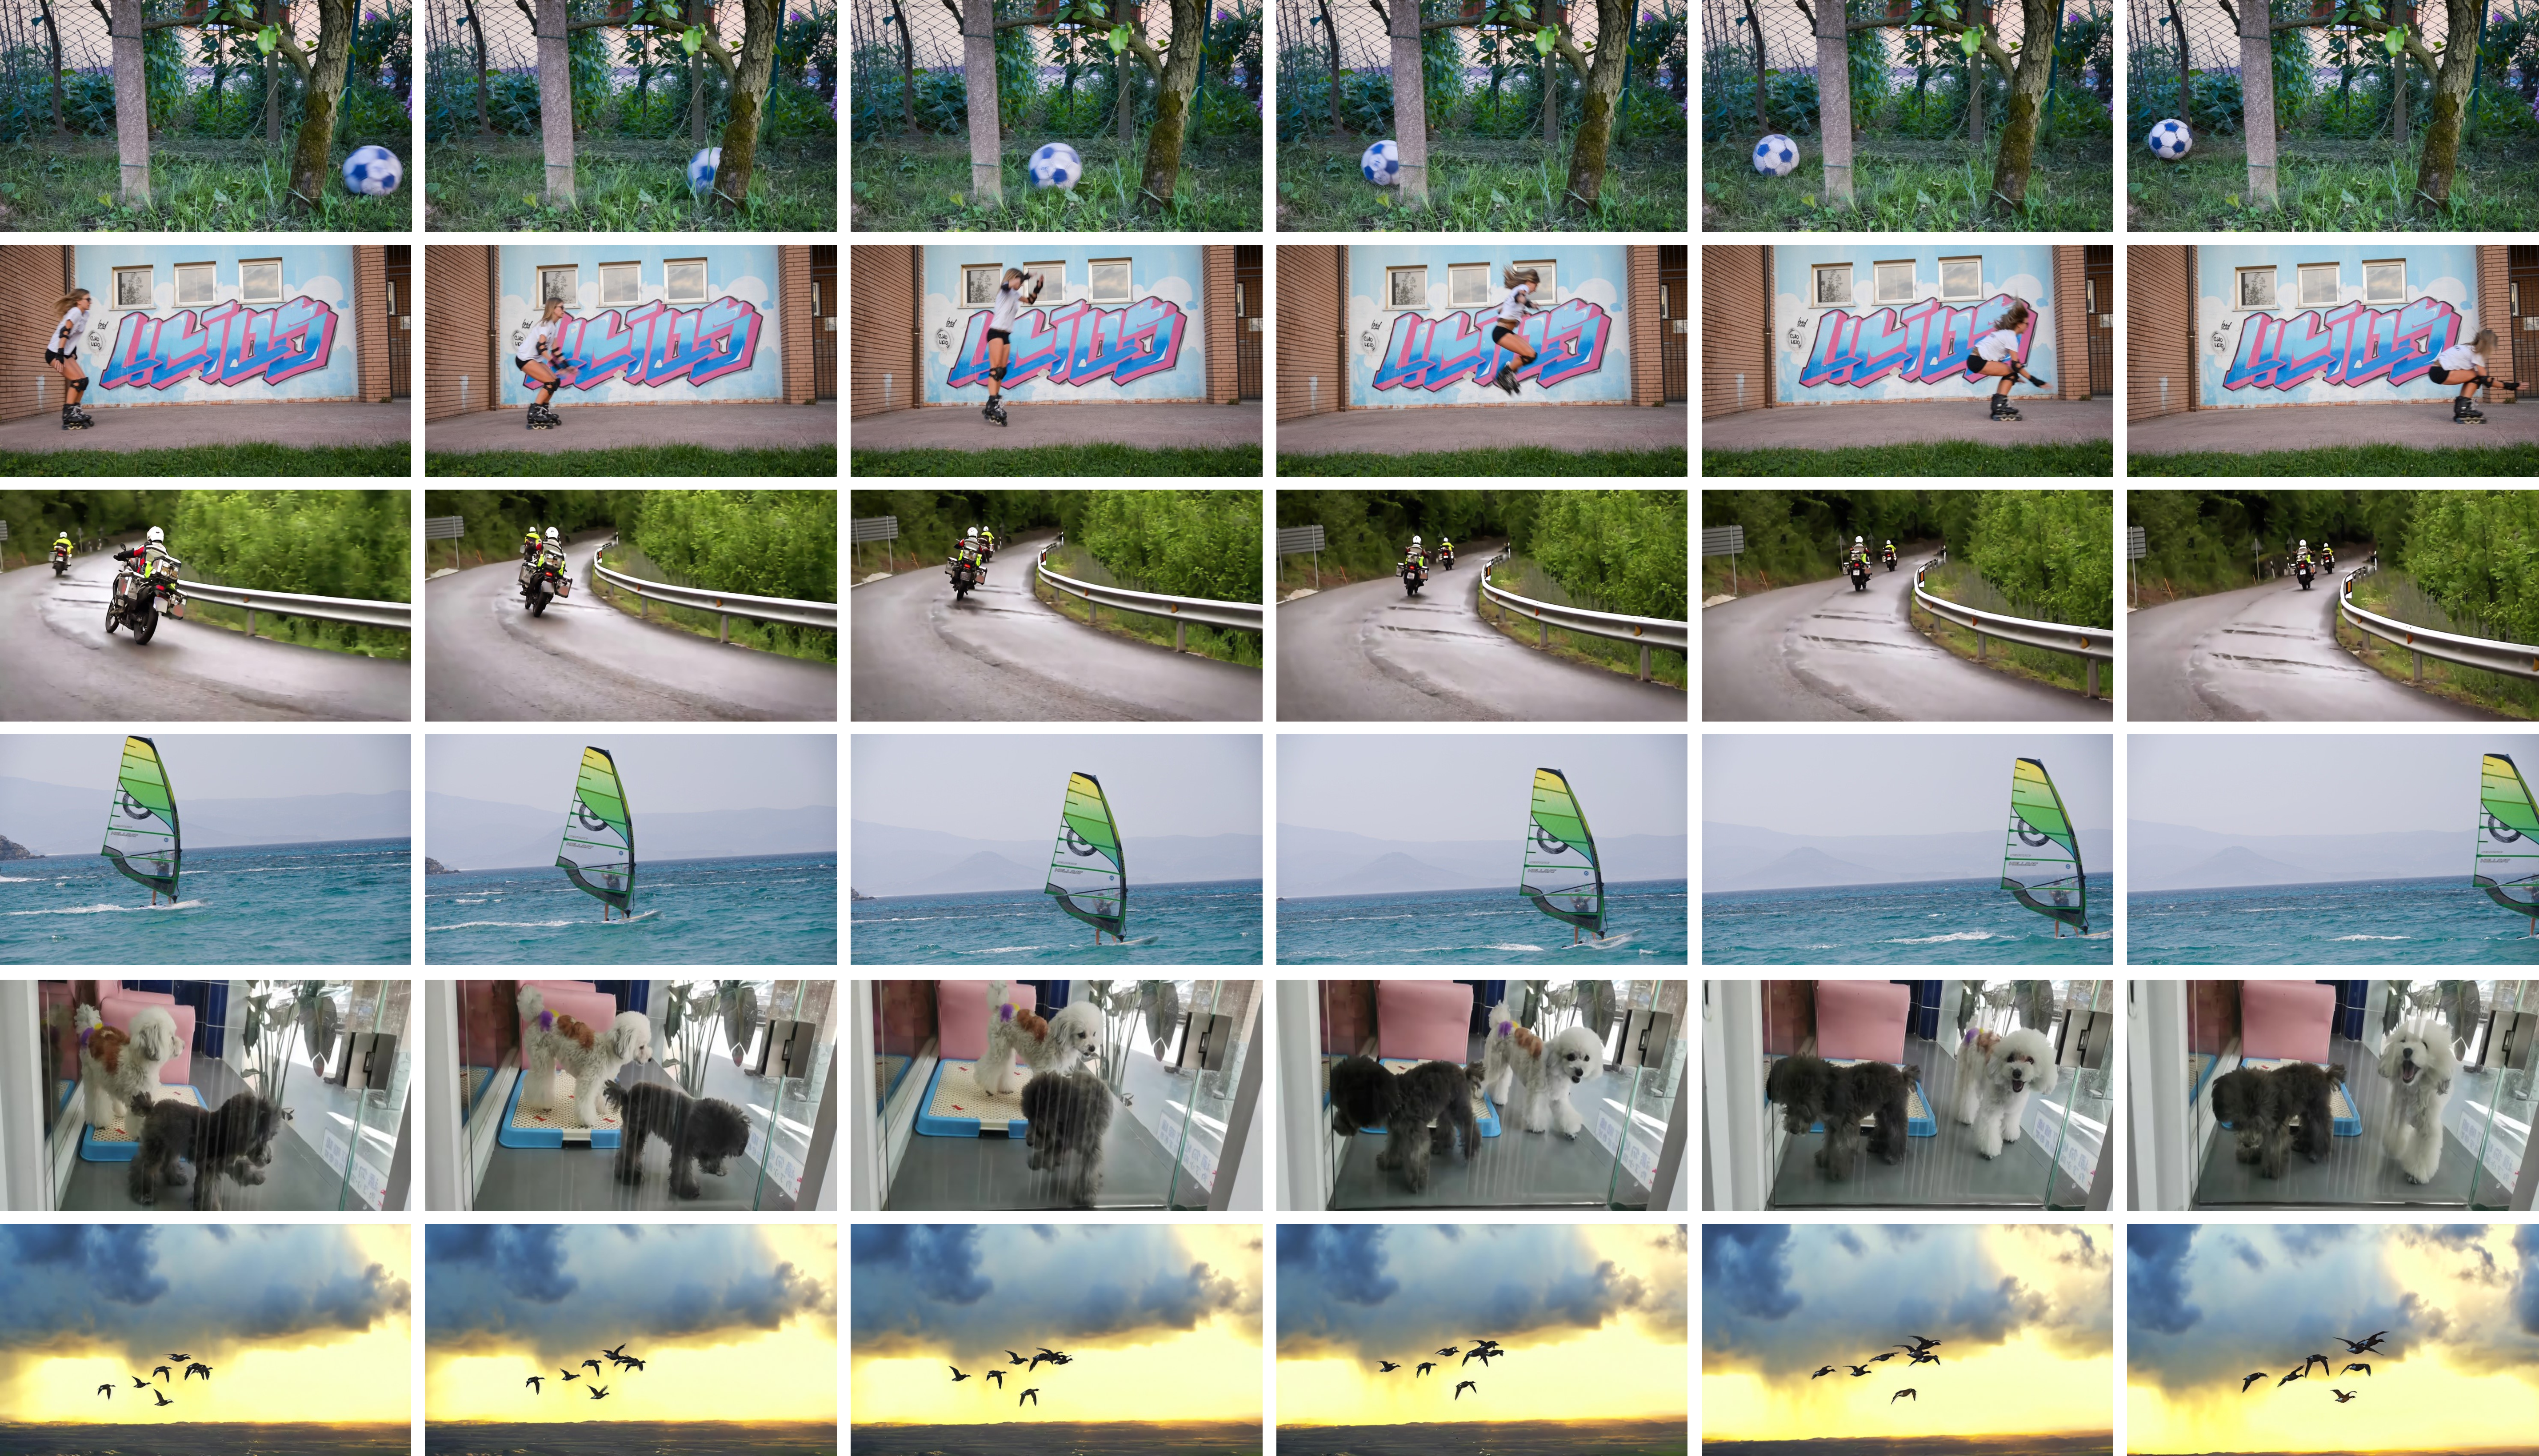
\includegraphics[width=\textwidth]{images/eval_data.pdf}
    \caption{
       Visualization of Our Evaluation Dataset, highlighting 0\%, 20\%, 40\%, 60\%, 80\%, and 100\% of the total duration. Each center point of the annotated object masks is treated as a trajectory point. The number of trajectories in the tested video matches the number of annotated objects.
    }
    \label{sup.f.eval}   
\end{figure*}

Drawing inspiration from OpenSora, we employ a multi-scale and mixed-duration training strategy, which involves training videos of various resolutions and lengths together. Specifically,we establish predefined buckets, each defined by a unique combination of (video resolution, duration). Videos are then assigned to the appropriate bucket according to their specific attributes. Note that videos of any aspect ratio will fall into these buckets if their total pixel count is within the specified statistical intervals. The parameter settings for the buckets adhere to the principle that lower resolutions correspond to longer durations, enabling Tora to adapt to videos of varying lengths. Notably, our preprocessing steps ensure that the shorter edge of each training video exceeds 720 pixels. To enable training across various scales, we shuffle the dataset and randomly select videos for downsampling to lower resolutions. Additionally, we employ different batch sizes for each bucket to balance the GPU load. The details of the buckets are presented in Figure~\ref{sup.f.bucket}.




\subsection{Evaluation Data}

Our evaluation dataset is primarily sourced from video object segmentation datasets~\cite{yt2021,qi2022occluded,pont2017}, which offer robust object motion critical for our analysis. To enhance the quality of our evaluation, we implement a camera motion filtering technique to select videos where the camera remains predominantly stable. This filtering process allows us to concentrate on where object motion is distinctly pronounced, thereby improving the reliability of our assessments. For each frame, we utilize the center of the annotated object masks as trajectory points, providing precise references for evaluating motion dynamics. Figure~\ref{sup.f.eval} presents several examples from our evaluation dataset, highlighting the diversity and relevance of the selected video sequences.

% \begin{figure}[!ht]
%     \centering
%     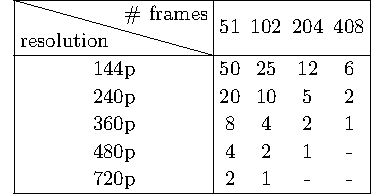
\includegraphics[width=0.47\textwidth]{images/bucket.pdf}
%     \caption{Batchsize for every bucket}
%     \label{sup.f.bucket}   
% \end{figure}






\section{Prompt Refinement}\label{sup.prompt}
We encourage users to provide detailed text prompts to achieve satisfactory video results. To ensure consistency in the distribution of text prompts during both training and testing phases, we utilize GPT-4o to refine simple testing prompts. The process of learning refined prompts for GPT-4o involves two key components. The first component is the task description, which clearly outlines the objectives for the model in generating enhanced content:

\texttt{You need to refine user's input prompt. The user's input prompt is used for video generation task. You need to refine the user's prompt to make it more suitable for the task. Here are some examples of refined prompts: $\downarrow$ \\ 
a close-up shot of a woman applying makeup. she is using a black brush to apply a dark powder to her face. the woman has blonde hair and is wearing a black top. the background is black, which contrasts with her skin tone and the makeup. the focus is on her face and the brush, with the rest of her body and the background being out of focus. the lighting is soft and even, highlighting the texture of the makeup and the woman's skin. there are no texts or other objects in the video. the woman's expression is neutral, and she is looking directly at the camera. the video does not contain any action, as it is a still shot of a woman applying makeup. the relative position of the woman and the brush is such that the brush is in her hand and is being used to apply the makeup to her face. the video does not contain any other objects or actions. the woman is the only person in the video, and she is the main subject. the video does not contain any sound. the description is based on the visible content of the video and does not include any assumptions or interpretations. $\downarrow$ \\
a professional setting where a woman is presenting a slide from a presentation. she is standing in front of a projector screen, which displays a bar chart. the chart is colorful, with bars of different heights, indicating some sort of data comparison. the woman is holding a pointer, which she uses to highlight specific parts of the chart. she is dressed in a white blouse and black pants, and her hair is styled in a bun. the room has a modern design, with a sleek black floor and a white ceiling. the lighting is bright, illuminating the woman and the projector screen. the focus of the image is on the woman and the projector screen, with the background being out of focus. there are no texts visible in the image. the relative positions of the objects suggest that the woman is the main subject of the image, and the projector screen is the object of her attention. the image does not provide any information about the content of the presentation or the context of the meeting. $\downarrow$ \\
a serene scene in a park. the sun is shining brightly, casting a warm glow on the lush green trees and the grassy field. the camera is positioned low, looking up at the towering trees, which are the main focus of the image. the trees are dense and full of leaves, creating a canopy of green that fills the frame. the sunlight filters through the leaves, creating a beautiful pattern of light and shadow on the ground. the overall atmosphere of the video is peaceful and tranquil, evoking a sense of calm and relaxation. $\downarrow$ \\
a moment in a movie theater. a couple is seated in the middle of the theater, engrossed in the movie they are watching. the man is dressed in a casual outfit, complete with a pair of sunglasses, while the woman is wearing a cozy sweater. they are seated on a red theater seat, which stands out against the dark surroundings. the theater itself is dimly lit, with the screen displaying the movie they are watching. the couple appears to be enjoying the movie, their attention completely absorbed by the on-screen action. the theater is mostly empty, with only a few other seats visible in the background. the video does not contain any text or additional objects. the relative positions of the objects are such that the couple is in the foreground, while the screen and the other seats are in the background. the focus of the video is clearly on the couple and their shared experience of watching a movie in a theater. $\downarrow$ \\
a scene where a person is examining a dog. the person is wearing a blue shirt with the word "volunteer" printed on it. the dog is lying on its side, and the person is using a stethoscope to listen to the dog's heartbeat. the dog appears to be a golden retriever and is looking directly at the camera. the background is blurred, but it seems to be an indoor setting with a white wall. the person's focus is on the dog, and they seem to be checking its health. the dog's expression is calm, and it seems to be comfortable with the person's touch. the overall atmosphere of the video is calm and professional. $\downarrow$ \\
The refined prompt should pay attention to all objects in the video. The description should be useful for AI to re-generate the video. The description should be no more than six sentences. The refined prompt should be in English.}

Following that, GPT-4o is supplied with the testing captions for processing. This allows it to refine the prompts based on the initial task description, ensuring that the provided captions are more detailed and aligned with our objectives:

\texttt{Generate the refined prompts for following inputs: $\downarrow$ \\
A man rides on a huge fish, flying from the water into the sky. $\downarrow$ \\
Two Jedi cats are fighting with each other in the forest. $\downarrow$  \\
A polar bear with a black hat is walking on the Great Wall. $\downarrow$  \\
A woman and a golden retriever are playing on the beach at sunset. $\downarrow$ \\
Two roses sway together before a snow-covered mountain range.
}

\section{Motion VAE Training}
Given the absence of pre-existing networks tailored for video optical flow compression, training such a network from scratch presents significant challenges. Directly transferring the motion vectors to the image domain and applying a pretrained 3D VAE may hinder the model's ability to effectively encode motion features, primarily due to domain discrepancies. To overcome this issue, we refine a motion-specific 3D VAE that is initialized from a pretrained model. Specifically,  our motion 3D VAE is specifically initialized using the architecture of OpenSora's VAE, which adapts the structure of Magvit-v2. This VAE has a substantial parameter count of 384 million, effectively leveraging the capabilities of a well-established network.  Our training data is sourced from a combination of datasets annotated with optical flow information~\cite{DBLP:conf/cvpr/MehlSJNB23,DBLP:conf/cvpr/MayerIHFCDB16,DBLP:journals/ijcv/RanjanHTTRB20,DBLP:journals/corr/abs-2001-10773}. We fine-tune the motion 3D VAE for 200,000 iterations with a batch size of 1. The training video size is set to a random number of frames, capped at 34. This setting aligns with the OpenSora video VAE, improving compatibility between the motion VAE and the video VAE and ensuring a cohesive training process. We utilize PSNR, SSIM and Trajectory Error to evaluate reconstruction quality and motion-controllable ability. The performance differences between the pure video VAE and our fine-tuned model are presented in Table~\ref{sup.t.vae}.

\begin{table}[!ht]
\centering
\begin{tabular}{cccc}
\toprule
Model          & PSNR$\uparrow$  & SSIM$\uparrow$  & TrajError$\downarrow$ \\ 
\midrule
Pure Video VAE & 27.34 & 0.842 & 17.09     \\
Our VAE        & 28.76 & 0.860 & 14.25     \\ 
\bottomrule
\end{tabular}
\caption{The performance comparison of different 3D VAE.}
\label{sup.t.vae} 
\end{table}
